%%%%%%%%%%%%%%%%%%%%%%%%%%%%%%%%%%%%%%%%%%%%%%%%%%%%%%%%%%%%%%%%
%  Scribe notes for MATH 279
%  William Yao
%%%%%%%%%%%%%%%%%%%%%%%%%%%%%%%%%%%%%%%%%%%%%%%%%%%%%%%%%%%%%%%%

\documentclass[11pt]{article}

\usepackage{amsmath,amssymb,amsrefs}
\usepackage{color}
\usepackage{amscd}
\usepackage{latexsym}
\usepackage{graphics}
\usepackage{framed}
\usepackage{url}
\usepackage{hyperref}
\usepackage{algorithm}
\usepackage{algorithmic}
\usepackage[compact]{titlesec}
\titlespacing{\section}{0pt}{0pt}{0pt}

\setlength{\oddsidemargin}{0.25 in}
\setlength{\evensidemargin}{-0.25 in}
\setlength{\topmargin}{-0.6 in}
\setlength{\textwidth}{6.5 in}
\setlength{\textheight}{9 in}
\setlength{\headsep}{0.4 in}
\setlength{\parindent}{0 in}
\setlength{\parskip}{0.1 in}

\usepackage{subfigure}
\usepackage{graphicx}

\newcommand{\remove}[1]{}

\newcommand{\lecture}[5]{
	\pagestyle{headings}
	\thispagestyle{plain}
	\newpage
	\noindent
	\begin{center}
		\framebox{
			\vbox{
				\hbox to 6.28in { {\bf MATH 279: Data Science and Machine Learning for Finance
						\hfill  - Winter 2026} }
				\vspace{4mm}
				\hbox to 6.28in { {\Large \hfill Lecture #1: #3  \hfill} }
				\vspace{2mm}
				\hbox to 6.28in { {\it Lecturer: #4 \hfill Scribe: #5} }
			}
		}
	\end{center}
	\markboth{Lecture #1: #3}{Lecture #1: #3}
   {\bf Disclaimer}: {\it These notes have not been subjected to the usual scrutiny reserved for formal publications. Nevertheless, they should give a fairly detailed account of the topics covered during the lecture. If you come across any mistakes or typos, please let us know.}
	\vspace*{4mm}
}
\newcommand\mydef{\mathrel{\overset{\makebox[0pt]{\mbox{\normalfont\tiny\sffamily def}}}{=}}}

\newcommand{\topic}[2]{\section{#1} \index{#2} \markright{#1}}
\newcommand{\subtopic}[2]{\subsection{#1} \index{#2}}
\newcommand{\subsubtopic}[2]{\subsubsection{#1} \index{#2}}

\renewcommand{\cite}[1]{[#1]}

\newcommand{\bi}{\begin{itemize}}
\newcommand{\ei}{\end{itemize}}
\newcommand{\be}{\begin{enumerate}}
\newcommand{\ee}{\end{enumerate}}
\newcommand{\blank}{\vspace{1ex}}
\newcommand{\mb}[1]{\mbox{\boldmath$#1$}}

\newtheorem{theorem}{Theorem}
\newtheorem{lemma}[theorem]{Lemma}
\newtheorem{claim}[theorem]{Claim}
\newtheorem{corollary}[theorem]{Corollary}
\newcommand{\qed}{\hfill $\Box$}
\newenvironment{proof}{{\em Proof:}}{\hfill\rule{2mm}{2mm}}

\newenvironment{dfn}{{\vspace*{1ex} \noindent \bf Definition }}{\vspace*{1ex}}
\newcommand{\bigdef}[2]{\index{#1}\begin{dfn} {\rm #2} \end{dfn}}
\newcommand{\smalldef}[1]{\index{#1} {\em #1}}

\begin{document}
\lecture{19--20}{}{Cluster-driven Hierarchical Representation of Large Asset Universes for Optimal Portfolio Construction}{Mihai Cucuringu}{William Yao}

\section{Introduction and Motivation}

The lecture studied how to make Markowitz portfolio construction more stable in a large asset universe. In the classical mean-variance framework, one seeks portfolio weights $\boldsymbol{\omega} \in \mathbb{R}^n$ that minimize risk subject to a target return:
\begin{equation*}
\left\{
\begin{array}{ll}
\underset{\boldsymbol{\omega}}{\min} & \boldsymbol{\omega}^{T}\boldsymbol{\Sigma}\boldsymbol{\omega} \\
\text{s.t.} & \boldsymbol{\omega}^{T}\bar{r} \geq \rho_0, \\
& \sum_{i=1}^{n} \omega_i = 1.
\end{array}
\right.
\end{equation*}
Here $\bar{r}$ is the vector of expected returns, $\boldsymbol{\Sigma}$ is the covariance matrix, and $\rho_0$ is the target return level.

The main issue emphasized in class is that this optimization becomes fragile when the number of assets is large. Empirical covariance matrices can be ill-conditioned, difficult to invert, and highly sensitive to noise when the number of historical observations is not much larger than the number of assets. This leads to unstable portfolio weights and poor out-of-sample performance.

The proposed solution is to introduce a hierarchical representation of the asset universe. Instead of optimizing directly over hundreds of assets, one first clusters similar assets, interprets each cluster as a synthetic asset, performs Markowitz optimization on that reduced universe, and then maps the cluster weights back to the original assets. The key idea is that clustering acts as a dimension reduction step while still retaining all constituent assets.

Relative to earlier cluster-based portfolio methods, this approach is more hierarchical. Rather than choosing a single representative stock from each cluster, it keeps all assets and assigns them intra-cluster weights. This preserves diversification while simplifying the covariance estimation problem.

\section{Graph-Based View of the Asset Universe}

To cluster assets, the lecture represents the market as a signed graph. Each node corresponds to an asset, and edge weights measure similarity between assets via their correlations. If asset $i$ has return vector $\mathbf{r}^{(i)} = [r^{(i)}_1,\ldots,r^{(i)}_d]^T$, the similarity between assets $i$ and $j$ is defined using the Pearson correlation
\begin{equation*}
\gamma_{ij} =
\frac{\sum_{k=1}^{d}(r^{(i)}_k-\bar{r}^{(i)})(r^{(j)}_k-\bar{r}^{(j)})}
{\sqrt{\sum_{l=1}^{d}(r^{(i)}_l-\bar{r}^{(i)})^2}
\sqrt{\sum_{m=1}^{d}(r^{(j)}_m-\bar{r}^{(j)})^2}} \in [-1,1].
\end{equation*}
The adjacency matrix of the graph is therefore the empirical correlation matrix $\Gamma = (\gamma_{ij})$.

This graph is signed because negative correlations are allowed. Positive edges indicate assets that tend to move together, while negative edges indicate assets that move in opposite directions. This makes signed graph clustering a natural tool: one wants strong positive dependence within clusters and weaker, or even negative, dependence across clusters.

The lecture briefly reviewed several signed spectral clustering ideas, including Signed Laplacian methods and SPONGE-type approaches. The main practical message was not the precise derivation of every algorithm, but rather why signed methods matter. Since correlation matrices naturally contain both positive and negative values, signed clustering methods can use more information than approaches that simply discard the sign structure.

\begin{figure}[h!]
\begin{center}
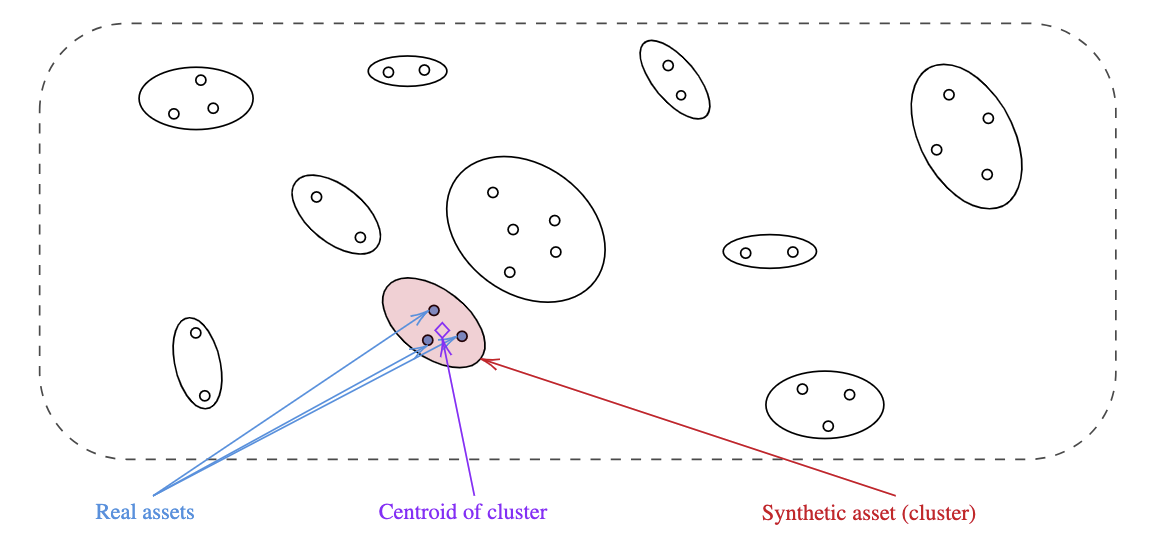
\includegraphics[width=0.58\columnwidth]{figs/synthetic_universe.png}
\end{center}
\caption{Clustering transforms a large asset universe into a smaller synthetic universe while preserving within-cluster structure.}
\end{figure}

\section{Cluster-Driven Hierarchical Portfolio Construction}

Once the signed graph is partitioned into $K$ clusters $\mathcal{C}_1,\ldots,\mathcal{C}_K$, each cluster is treated as a synthetic asset. The resulting reduced universe has size $K \ll n$, which makes covariance estimation and optimization more manageable. The cluster-level Markowitz problem becomes
\begin{equation*}
\left\{
\begin{array}{ll}
\underset{\boldsymbol{\omega}^{*}}{\min} & \boldsymbol{\omega}^{*T}\boldsymbol{\Sigma}^{*}\boldsymbol{\omega}^{*} \\
\text{s.t.} & \boldsymbol{\omega}^{*T}\bar{r}^{*} \geq \rho_0, \\
& \sum_{i=1}^{K} \omega_i^{*} = 1.
\end{array}
\right.
\end{equation*}
Here $\bar{r}^{*}$ and $\boldsymbol{\Sigma}^{*}$ are the expected return vector and covariance matrix for the synthetic assets.

The lecture then described how cluster-level quantities are constructed. If asset $i$ belongs to cluster $k$, it receives an intra-cluster weight $\beta_{i,k}$. The synthetic return and expected return of cluster $k$ are
\begin{equation*}
r_k^{*} = \sum_{i=1}^{n}\beta_{i,k} r_i \mathbf{1}_{(A^{(i)}=k)},
\qquad
\bar{r}_k^{*} = \sum_{i=1}^{n}\beta_{i,k} \bar{r}_i \mathbf{1}_{(A^{(i)}=k)}.
\end{equation*}
The covariance matrix $\boldsymbol{\Sigma}^{*}$ is then computed from these synthetic returns, after which Markowitz optimization yields extra-cluster weights $\alpha_1,\ldots,\alpha_K$.

Finally, the portfolio weight of each original asset is obtained by combining the cluster weight with the within-cluster weight:
\begin{equation*}
\omega_i = \alpha_{A^{(i)}} \beta_{i,A^{(i)}}.
\end{equation*}
This formula shows the hierarchical structure clearly: the optimization first allocates capital across clusters, then distributes capital within each cluster.

The lecture also discussed an ensembling step. Since some clustering methods involve randomness, the clustering and portfolio construction stages can be repeated multiple times inside the same trading window, and the resulting portfolios can be averaged. This reduces sensitivity to the specific random initialization of the clustering routine.

\section{Key Modeling Choices and Parameters}

\subsection{Gaussian Constituent Weights}

Instead of selecting a single representative asset per cluster, the method assigns weights to all assets according to their distance from the cluster centroid $\mu_k$. The intra-cluster weights are defined through a Gaussian kernel:
\begin{equation*}
\beta_{i,k} =
\frac{\exp\left(-\frac{\lVert \mathbf{r}^{(i)} - \mu_k \rVert^2}{2\sigma^2}\right)}
{\sum_{j \in \mathcal{C}_k} \exp\left(-\frac{\lVert \mathbf{r}^{(j)} - \mu_k \rVert^2}{2\sigma^2}\right)}.
\end{equation*}
Here $\sigma^2$ is a bandwidth parameter controlling how concentrated the weights are around the cluster center. Intuitively, assets closer to the cluster centroid receive larger weights, but all assets in the cluster still contribute.

\subsection{Synthetic Return Forecasting}

Because the quality of expected return estimates strongly affects Markowitz portfolios, the lecture introduced a simple way to study prediction quality without claiming to solve the forecasting problem itself. A parameter $\eta$ measures the quality of the return prediction, with larger $\eta$ corresponding to stronger correlation between the true future return signal and the noisy forecast used in optimization.

This construction is mainly a device for sensitivity analysis. It allows one to ask how much the clustering framework benefits from better forecasts, without tying the lecture to a specific predictive model.

\subsection{Choosing the Number of Clusters}

The lecture proposed choosing the number of clusters by a PCA-style cumulative variance rule. If $\lambda_1 \geq \cdots \geq \lambda_n$ are eigenvalues of the relevant matrix, choose the smallest $k$ such that
\begin{equation*}
\frac{\sum_{i=1}^{k}\lambda_i}{\sum_{i=1}^{n}\lambda_i} \geq P,
\end{equation*}
where $P$ is a prescribed variance threshold. In the empirical analysis, this pointed toward cluster counts such as $10$ and $24$, which are also economically meaningful because they align with levels of the GICS industry hierarchy.

\begin{figure}[h!]
\begin{center}
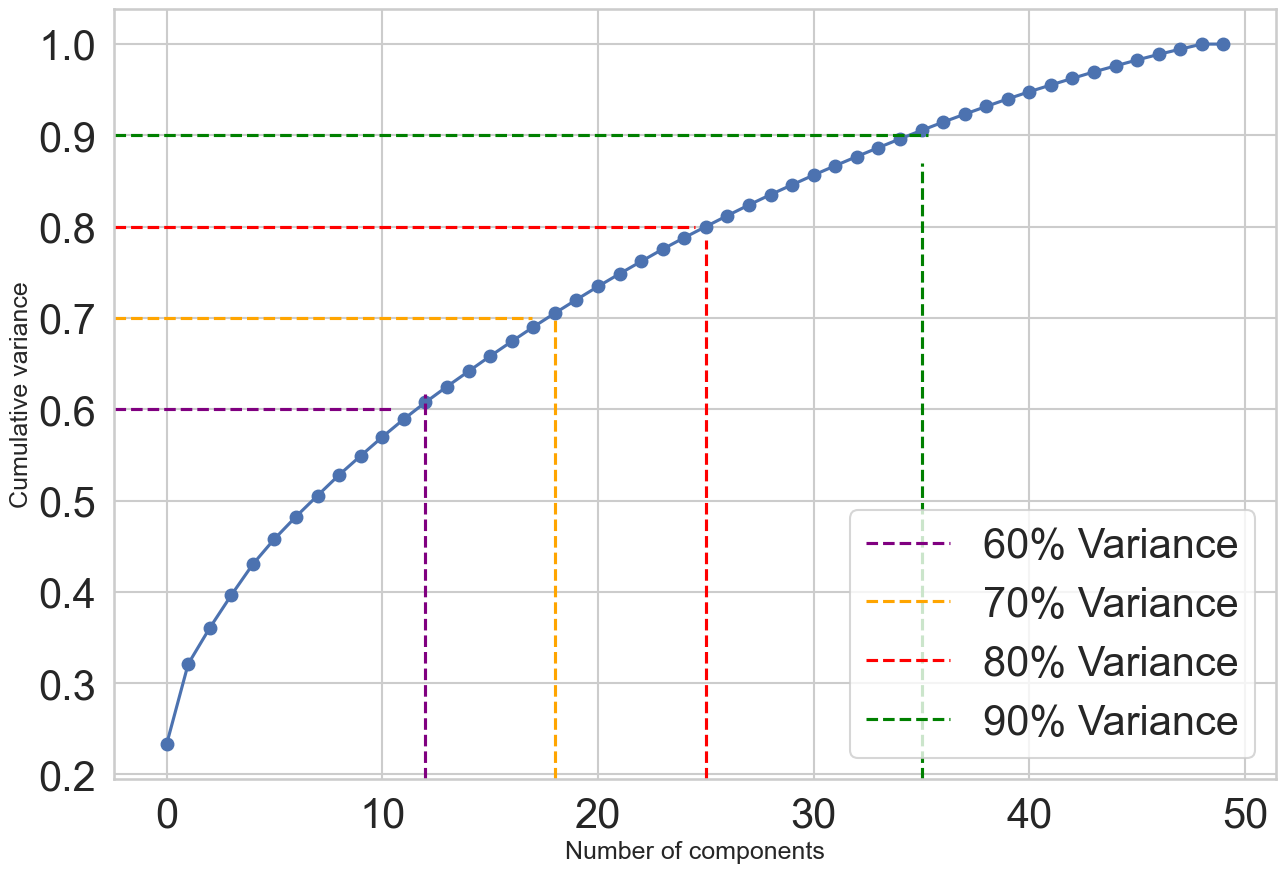
\includegraphics[width=0.50\columnwidth]{figs/pca_clusters.png}
\end{center}
\caption{A PCA-style cumulative variance criterion can guide the choice of the number of clusters.}
\end{figure}

\subsection{Turnover, Transaction Costs, and EWA Covariance}

The lecture also emphasized that realistic performance evaluation must include trading frictions. If $V_t$ is the portfolio value at time $t$, then turnover is
\begin{equation*}
TO_t = \sum_{i=1}^{n}|T_{t,i}| = V_t \sum_{i=1}^{n}|w_{t,i} - w_{t-1,i}|.
\end{equation*}
With a proportional transaction cost rate $\tau_{\text{transac}}$, the net profit and loss is
\begin{equation*}
\text{PnL}_{t,\text{net}} = \text{PnL}_{t,\text{initial}} - \tau_{\text{transac}} TO_t.
\end{equation*}
An important practical conclusion from the slides is that transaction costs matter much more at daily rebalancing frequencies than at weekly frequencies.

To address the non-stationarity of financial returns, the lecture replaced the ordinary sample covariance with an exponentially weighted average (EWA) covariance matrix:
\begin{equation*}
\mathbf{E} = \frac{1-\beta}{1-\beta^d}\sum_{t=1}^{d}\beta^{d-t} x_t^T x_t,
\end{equation*}
where $\beta \in (0,1)$ is a decay parameter and $x_t$ denotes the cross-section of returns at time $t$. This gives greater emphasis to recent observations and is motivated by volatility clustering in financial data.

\section{Empirical Findings and Interpretation}

The empirical backtest compared several naive strategies with the proposed cluster-driven approaches on a large universe of U.S. equities. The baselines included an equally weighted portfolio, a naive Markowitz portfolio on the full universe, and an S\&P 500 benchmark. The central question was whether clustering before optimization improves performance.

The answer from the lecture was clearly yes. Across the reported experiments, cluster-based strategies generally achieved lower volatility and better risk-adjusted returns than the naive Markowitz strategy. In particular, signed clustering methods outperformed plain spectral clustering on the absolute-value correlation matrix, suggesting that negative correlations contain useful information for portfolio construction.

\begin{figure}[h!]
\begin{center}
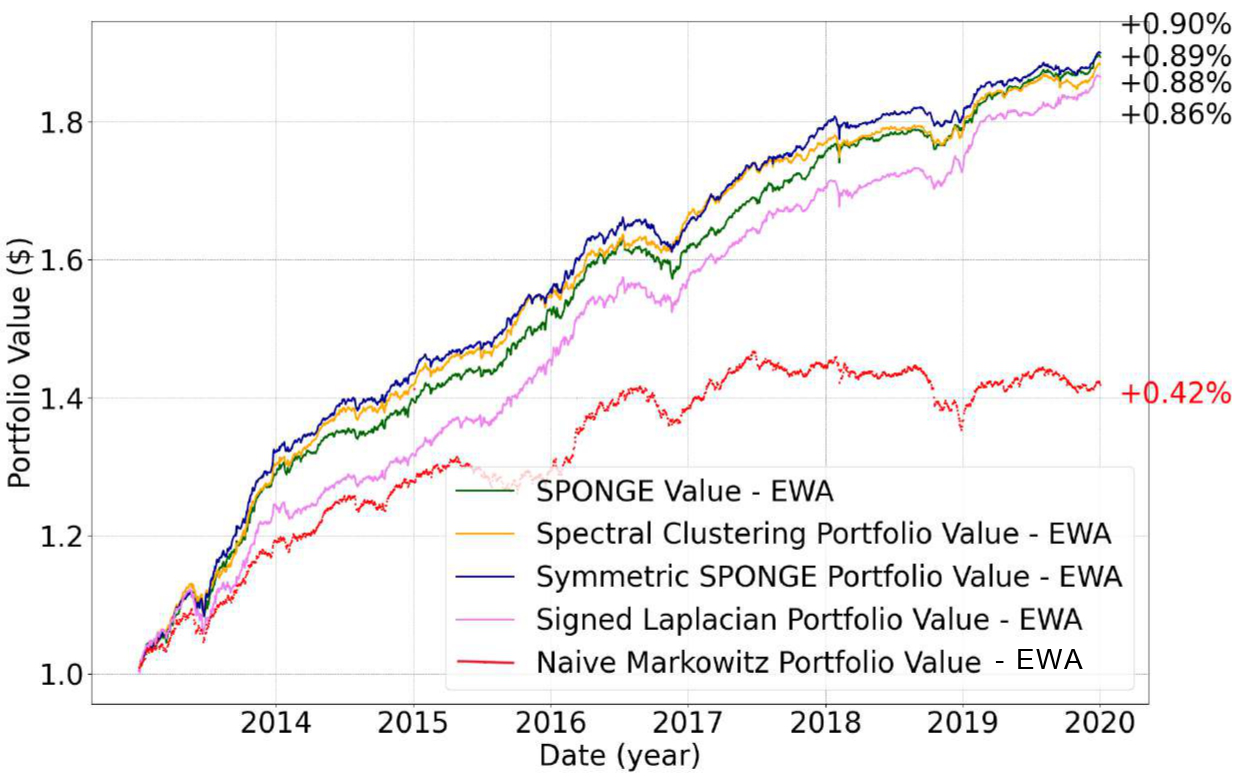
\includegraphics[width=0.82\columnwidth]{figs/ewa_strats.png}
\end{center}
\caption{Cluster-driven strategies with EWA covariance outperform naive Markowitz in cumulative portfolio value.}
\end{figure}

Several comparative conclusions were emphasized in class.
\begin{itemize}
\item Naive Markowitz tends to have the worst volatility metrics among the optimization-based strategies, reflecting the instability of covariance estimation in high dimensions.
\item Adding the clustering layer reduces effective dimension and improves the quality of the optimization problem.
\item Incorporating EWA covariance estimation further improves performance by adapting to non-stationarity.
\item Signed clustering methods, especially SPONGE-type variants, attain the strongest Sharpe and Sortino ratios in the reported experiments.
\end{itemize}

The lecture also examined sensitivity to the number of clusters $K$. Among the tested values, $K=24$ gave the best overall balance of return and volatility. One interpretation discussed in class is that $24$ clusters preserve enough information while still matching a meaningful economic partition of the market through the GICS industry-group structure. By contrast, very small $K$ may over-compress the universe and discard useful information.

Finally, the lecture studied sensitivity to prediction quality through the parameter $\eta$. As $\eta$ increases, portfolio performance improves substantially, both in return and in risk-adjusted terms. Even so, the cluster-based strategies remain competitive relative to naive Markowitz when prediction quality is low, which suggests that the hierarchical representation itself already contributes meaningful robustness.

\section{Research Directions and Open Questions}

The lecture concluded by stressing that this framework is flexible rather than final. Several research directions arise naturally from the material.

\begin{itemize}
\item \textbf{Alternative similarity measures.} Pearson correlation is convenient, but other dependence measures may better capture nonlinear comovements or tail dependence across assets.
\item \textbf{Alternative clustering methods.} The performance gap between signed clustering algorithms suggests that clustering quality matters. It would be valuable to understand when particular signed methods are most effective.
\item \textbf{Within-cluster optimization.} Instead of assigning intra-cluster weights only through a Gaussian kernel, one could run a second optimization problem inside each cluster and compare the resulting portfolios.
\item \textbf{Better covariance forecasting.} EWA is a simple way to address non-stationarity, but richer covariance models such as GARCH-type, factor-based, or deep learning methods may improve the synthetic covariance matrix further.
\item \textbf{Forecast uncertainty and robustness.} Since performance depends strongly on the prediction quality parameter $\eta$, a natural next step is to incorporate explicit uncertainty quantification into the portfolio optimization stage.
\item \textbf{Economic interpretation of the hierarchy.} The good performance of $K=24$ raises the question of whether optimal clusters should be chosen statistically, economically, or through some hybrid criterion combining both.
\end{itemize}

More broadly, the lecture suggests an appealing research theme: rather than viewing clustering as a preprocessing trick, one can treat it as a structural representation of the market that changes the geometry of the portfolio optimization problem itself.

\end{document}
